% !TEX root = ../lectures_olympics.tex

\chapter{静力学}

同学们可能有所耳闻,自然界中有四种基本的相互作用力,它们分别是万有引力、电磁力、强和弱相互作用力。
\emph{力(force)}是物体之间相互作用的一种表现形式,当有力作用在任何一个物体上时,它将会对力的作用产生响应,响应的形式有很多,其中最明显的就是运动状态或形状的改变。
我们将首先学习力的基本的一面,即如何对力进行测量,如何描写物质系统的受力,在已知力作用下处于静止状态力学系统的性质。
在随后的课程中将逐步深入,研究在已知的力作用下如何预测物体未来的运动的方法,从力的宏观性质出发进入到物质世界的深处进一步探索力的起源。


\section{力的基本性质}

对宏观物体受力的研究是学习描写各种力最初的一步,将来可以看到,这里所学的技术对于那些无法直观体验的对象之间相互作用的问题提供了丰富的术语和方法。
为了完整描写宏观物体所受的一个力,需要指出该力的大小、方向和作用在物体上的位置,也就是作用点,它们合起来称为力的三要素。
从更基本的观点来看,力可以用空间中的一个矢量来描写,力的三要素一起给出了作为一个矢量的大小、方向和起点的位置。
方向和作用点由传统的几何方法给出,而力的大小则需要引入一个新的单位,为了纪念力学的奠基人,今天将力的单位取为\emph{牛顿},用 N 来表示,将在动力学中给出其准确含义。

虽然从最基本的角度来看自然界只有四种相互作用力,而且强、弱相互作用只存在于亚原子物理当中,也就是说宏观物体的受力全部起源于万有引力和电磁相互作用力,原则上可以根据它们的性质以及物质的结构从微观理论出发预测出各种情况下宏观物体的受力。
但是实践上以这种方法得到宏观物体的受力实际上是不现实的,因为物质世界极大的复杂性。
所以在实际的研究过程中首先根据力的表现形式和效果对其进行分类,研究力和那此已知的、容易观察的物理量之间的关系,最后逐步地深入探讨力的本质和起源。
基于经验和观察人们发现了几种常见的力,下面我们逐一了解一下它们。

\subsection{重力}
本质上讲重力是万有引力在地球表面附近的一种表现形式,它来自于地球对所有物体的吸引。
观测表明,处于地球表面附近的物体都会受到重力作用,在地球的任何地方,其方向均竖直向下指向地面,大小正比于物体的质量,作用于物体的重心处。
关于重力有几点需要说明的地方:
\begin{itemize}
\item
将地表任何一点处物体所受重力大小$G$与其质量$m$的比例系数称为地表的\emph{重力加速度},用$g$表示
\begin{equation}
G = mg,\qquad g\approx 9.8\unit{m/s^2},
\end{equation}
\item
真实的测量表明地球各处的重力加速度大小几乎相同,但有细微的差别,造成这个判别的原因是地球的自转和形状,关于这一点需要在完整地学习了引力的性质以后才能得到答案。
\item
同样由于地球的自转和形状,重力的大小也不是完全垂直于地表,或者说不严格指向地心,但差别在一定情况下可以忽略不计。
\item
重心是重力的作用点,正常情况下一个物体的重心与其质心重合。
如果物体可以看成是由多个质点构成,将这些质点编号,第$i$个质量的质量为$m_i$,在固定的直角坐标系中的位置为$(x_i,y_i,z_i)$的时,质心的坐标$(x_c,y_c,z_c)$为
\begin{equation}
x_c=\frac{\sum_i m_ix_i}{\sum_i m_i},\qquad y_c=\frac{\sum_i m_iy_i}{\sum_i m_i},\qquad 
z_c=\frac{\sum_i m_iz_i}{\sum_i m_i}
\end{equation}

\end{itemize}

%%%%%%%%%%%%%%%%%
\begin{example}
求一块三边长分别为$a、b、c$的均匀三角板的重心位置。
\begin{flushright}
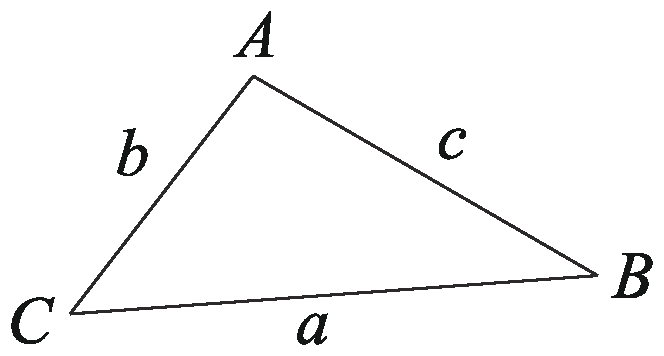
\includegraphics[width = 0.3\textwidth]{images/static-force-1.pdf} 
\end{flushright}

\tagged{student}{\vspace*{1cm}}
\begin{taggedblock}{teacher}
\vspace*{4cm}
\noindent
解析:初中学过三角形的重心,是从顶点到对边中点连线的交点。
这一结论对于均匀三角形板也是成立的。
\end{taggedblock}
\end{example}
%%%%%%%%%%%%%%%%%%%%%%


%%%%%%%%%%%%%%%%%
\begin{example}

求由三根据均匀杆构成的三角形的重心位置,其中三杆长度分别为$a、b、c$,满足$a^2+b^2=c^2$。
\begin{flushright}
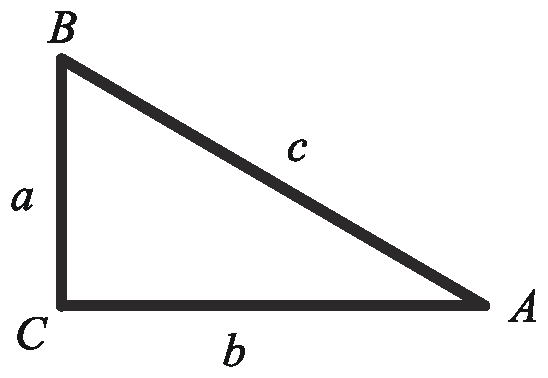
\includegraphics[width = 0.3\textwidth]{images/static-force-2.pdf} 
\end{flushright}
\tagged{student}{\vspace*{1cm}}
\begin{taggedblock}{teacher}
\vspace*{4cm}
\noindent
解析:建立坐标以$C$为原点的坐标系,那么重心的坐标
\begin{eqnarray*}
x_c\frac{b\times \frac{b}{2}+c\times\frac{b}{2}}{a+b+c},\qquad y_c  \frac{a\times \frac{a}{2}+c\times\frac{a}{2}}{a+b+c}
\end{eqnarray*}
\end{taggedblock}
\end{example}
%%%%%%%%%%%%%%%%%%%%%%



%%%%%%%%%%%%%%%%%
\begin{example}

求下面阴影的重心。
\begin{flushright}
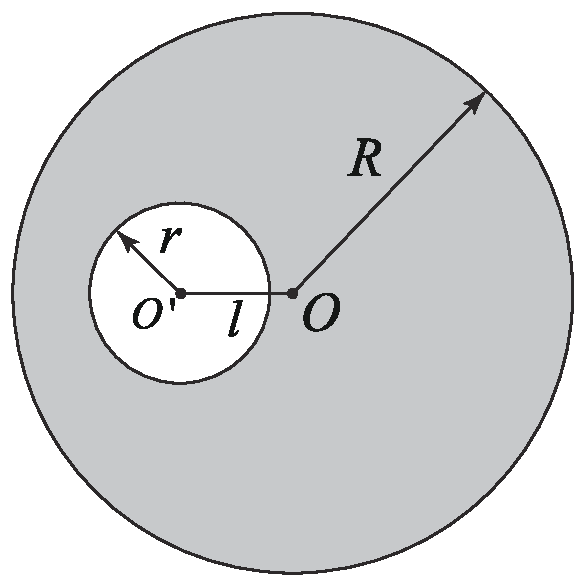
\includegraphics[width = 0.3\textwidth]{images/static-force-3.pdf} 
\end{flushright}
\tagged{student}{\vspace*{2cm}}
\begin{taggedblock}{teacher}
\noindent
解析:重心在对称轴上,把空白部分看成具有负的质量与完整的板构成的整体,那么重心在原点左边
\[
\frac{\pi r^2 l}{\pi R^2-\pi r^2} = \frac{r^2}{R^2-r^2}l
\]
\end{taggedblock}
\end{example}
%%%%%%%%%%%%%%%%%%%%%%


%%%%%%%%%%%%%%%%%
\begin{example}

已知一个质量为$M$的没有盖子的圆柱形的杯子。
里面开始是空的,然后往里面慢慢的注水。
进入了杯子的水和杯子的总重心会发生变化。
请问重心如何变化?是否有最值?是多少?
(已知杯子底面积为$S$,水的密度为$\rho$ ,原来空杯子重心高度为$H$)
\begin{taggedblock}{teacher}
\vspace*{4cm}
\newline
解析:建立竖直向上的坐标系,设水的高度为$h$,那么重心的位置与水面高度的关系为
\[
y_c(h) = \frac{\frac{1}{2}\rho S h^2+MH}{\rho S h + M}
\]
从中可看出重心先降低再升高,当
\[
h = \frac{\sqrt{M^2+2\rho SHM}-M}{\rho S}
\]
时重心位置最低。
\end{taggedblock}
\end{example}
%%%%%%%%%%%%%%%%%%%%%%


%%%%%%%%%%%%%%%%%
\begin{example}
【思考题】已知一个均匀质量的圆球壳,半径为$R$,现在将球壳上端高度为$h$ 的部分切下,然后粘贴在圆球的最下面,形成一个“杯子”。
求这个杯子的重心。

\tagged{student}{\vspace*{4cm}}
\begin{taggedblock}{teacher}


\end{taggedblock}
\end{example}
%%%%%%%%%%%%%%%%%%%%%%


\subsection{弹力}
当相互接触的物体发生形变时所产生的恢复形变的力称为弹性力,\emph{胡克定律}表明,当物体形变不太大时,弹性力与形变成正比,弹簧的弹性力$F$与弹簧相对于原长的形变(拉伸或压缩)$x$成正比,方向指向平衡位置,即
\begin{equation}
F = -kx,
\end{equation}
式中比例系数$k$称为弹簧的\emph{倔强系数},也叫\emph{劲度系数},负号表示弹性力与形变反方向。
关于弹力也有几点需要注意的地方:
\begin{itemize}
\item
当把多根弹簧并排放置共同作用时,称两弹簧\emph{并联},并联弹簧在任意位置处形变量相同。
很容易证明,多根弹簧并联的等效劲度系数
\begin{equation}
k = k_1+k_2+\cdots,
\end{equation}
为每根弹簧劲度系数之和。
和电路类比,除了并联以外多根弹簧之间也可以串联,处于串联状态的弹簧在受力以后形变量并不相同,但内部张力相同。
可以证明并联弹簧的等效劲度系数为
\begin{equation}
\frac{1}{k} = \frac{1}{k_1}+\frac{1}{k_2}+\cdots
\end{equation}
\item 
绳子的张力是一种弹性力,绳子和与之连接的物体之间有相互作用时,不仅绳子与物体之间有弹性力,而且在绳子内部也因发生相对形变而出现弹性力。
这时,绳子上任一横截面两边互施作用力,这对作用力和反作用力称为绳子的张力,一般情况下,与绳子相应的比例系数$k$很大,因而形变很小,可以忽略。
所以绳子的张力不是由绳子的形变规律确定,而是由求解力学问题时确定。
因而我们一般抽象出柔软不可伸长的轻绳。
\item
在光滑面(平面或曲面)上运动的物体受到的支撑力也是一种弹性力。
这种由物体与支撑面相互作用而发生形变产生的弹性力,也是一种使物体约束在该支撑面上运动的约束力,通常把物体所受到的约束力称为约束反力,约束反力的方向总是与支撑面垂直。
与绳子的张力一样,由于相应的$k$很大,因而形变很小,可以忽略,约束反力的大小由求解物体的运动来确定,若支撑面是粗糙的,则物体除受约束反力外,还要考虑该表面的摩擦力。
\item
所有弹力的起源均为电磁相互作用力,这一点只有从微观角度才能够发现。

\end{itemize}



%%%%%%%%%%%%%%%%%
\begin{example}
证明:串联弹簧的等效弹性系数小于其中任何一根弹簧的弹性系数,并解释形成这一现象的原因。
\tagged{student}{\vspace*{4cm}}
\begin{taggedblock}{teacher}
\newline
解析:串联的弹簧的总形变是每根弹簧形变量之和,而各个弹簧受力相同,所以等效弹性系数小于任何一根。
\end{taggedblock}
\end{example}
%%%%%%%%%%%%%%%%%%%%%%

\subsection{滑动摩擦力、静摩擦力}
\emph{摩擦力}也是一种接触力,当相互接触的物体作相对运动或有相对运动趋势时,接触面间会产生一种阻碍相对运动或相对运动趋势的力,这种力称为摩擦力,前者称为\emph{滑动摩擦力},后者称为\emph{静摩擦力}。
测量结果表明:
\begin{enumerate}
\item 滑动摩擦力与正压力成正比,与两物体的接触面积无关,与相对速度方向相反
\begin{equation}
f=-\mu N
\end{equation}
其中$\mu$称为动摩擦系数,多数情况下可以认为是一个常数。
\item 当相对速度不太大时,滑动摩擦力与速度无关
\item 静摩擦力的大小为0与最大值(称为最大静摩擦力)之间的某一值,此值由相对运动趋势的程度而定,最大静摩擦力也与正压力成正比。
最大静摩擦力
\begin{equation}\label{eqn: force-最大静摩擦}
f_{max}= \mu_0 N
\end{equation}
$\mu_0$称做\emph{静摩擦系数},它与动摩擦系数近似相等,统称为\emph{摩擦系数}。
\end{enumerate}


%%%%%%%%%%%%%%%%%
\begin{example}

如图所示,木板$A$质量为$M$,以相对地面的速度$v$在水平面上向北运动,木板上放一质量为$m$的板$B$ ,各接触面间滑动摩擦因数均为$\mu$,当木块$B$也有相对地面向东的速度$v$ 时,试分析木块$B$的受摩擦力的情况。
\begin{flushright}
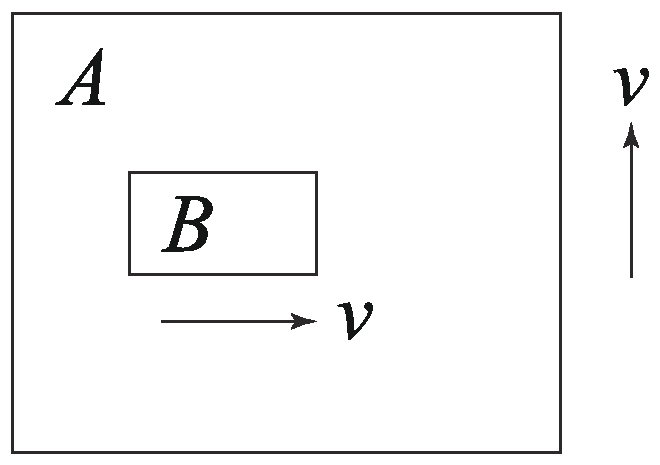
\includegraphics[width = 0.3\textwidth]{images/static-force-8.pdf} 
\end{flushright}
\tagged{student}{\vspace*{4cm}}
\begin{taggedblock}{teacher}
\vspace*{3cm}
\noindent
解析:相对于$A$,$B$的速度$\sqrt{2}v$向东南方向,因为滑动摩擦力与相对运动方向相反,所以$B$受到的摩擦力向西北方向,
\end{taggedblock}
\end{example}
%%%%%%%%%%%%%%%%%%%%%%


\section{受力分析}



当一个物体受多个力作用时,需要给定所有力的大小、方向和作用点才能够完全了解它的受力情况。
多个力作用的效果可以看成是一个\emph{合力}作用,如果各个力的方向都通过一个给定点,则称这几个力为共点力,共点力的合力为几个力的矢量和:
\begin{equation}
\vec{F} = \sum_i\vec{F}_i.
\end{equation}
当在坐标系中分析受力时,将一个给定的力向着坐标轴的方向分解对处理问题也是有帮助的。
一个力沿给定方向的分力的方向自然沿着那个已知的方向,而大小则是力本身的大小与力的方向与希望分解方向夹角余弦的乘积。



%%%%%%%%%%%%%%%%%
\begin{example}
如图所示,有五个力$\vec{F}_1,\vec{F}_2,\vec{F}_3,\vec{F}_4,\vec{F}_5$作用于一点$O$,构成一个正六边形的两邻边和三条对角线。
设$F_3 = 10\unit{N}$,试求这五个力的合力。
\begin{flushright}
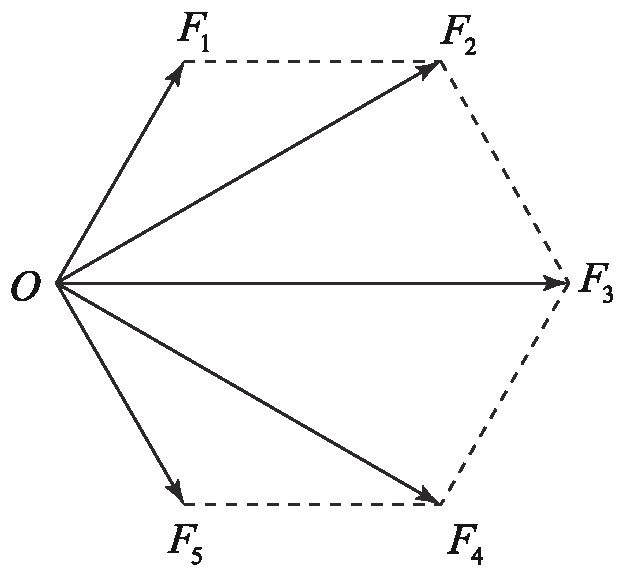
\includegraphics[width = 0.3\textwidth]{images/static-force-6.pdf} 
\end{flushright}

\tagged{student}{\vspace*{1cm}}
\begin{taggedblock}{teacher}
\noindent
解析:根据六边形的几何性质以及平行四边行法则可以得到,五个力的合力方向指向正右方,大小
\[
F = 2\cdot\frac{1}{2}F_3\cos\frac{\pi}{3}+2\cdot\frac{\sqrt{3}}{2}F_3\cos\frac{\pi}{6}+F_3 = 3F_3 = 30\unit{N}
\]
\end{taggedblock}
\end{example}
%%%%%%%%%%%%%%%%%%%%%%




找出力学系统中每个物体受力的大小、方向和作用点的过程称为受力分析,一般来说在静力学中主要考虑上面提到过的几种典型的受力。
除了特别的假设,地面附近所有物体都受重力,发生形变的弹性物体有弹力作用,相互接触的表面之间有可能有压力,当有压力并且有相对运动或相对运动趋势时还可能有摩擦力。
除此之外,在有的问题中还可能出现大气压力、浮力等其它种类的力,做受力分析的时候要把所有重要的因素全部考虑方可。

虽然力的效果在物理上是一致的,但不同的力也有细微的区别。
在做受力分析时,可以将力分为两大类,一类称做\emph{主动力},例如重力、弹簧弹力等。
这些力的共同特点就是它们可由系统的状态直接确定,只要知道了物体的质量、弹簧的弹性系数和形变量以后就可以确定其大小和方向。
另一类称\emph{约束力}或\emph{被动力},例如支持力、两个物体连接处的作用力等,它们无法直接确定,是由主动力和限制物体运动约束的性质共同决定。



%%%%%%%%%%%%%%%%%
\begin{example}

均匀长棒一端搁在地面上,另一端用细线系在天花板上,如图所示,若细线竖直,试分析棒的受力情况。
\begin{flushright}
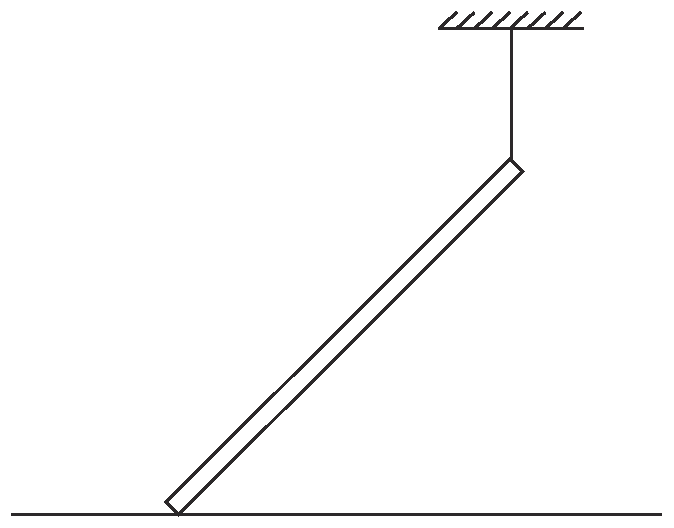
\includegraphics[width = 0.3\textwidth]{images/static-force-10.pdf} 
\end{flushright}
\tagged{student}{\vspace*{0cm}}
\begin{taggedblock}{teacher}
\noindent
解析:如上图所示。
\end{taggedblock}
\end{example}
%%%%%%%%%%%%%%%%%%%%%%









\section{静力平衡}

在多个力作用下处于平衡状态系统,所受到各个力的大小和方向必然有一定的联系。
因为力的效果总是使物体的运动状态发生变化,而处于静力平衡的物体的运动状态没有发生变化,所以它受到的合力必然为零。
对这一事实的描写有两种方式。
一种是直接的矢量计算,画出各个力的大小和方向,对于处于平衡状态系统中的每一个独立的部分,处于静力平衡时所受外力的矢量和必然为零,利用此方法更多地需要几何知识和技巧。
第二种常用的方法则是根据问题的特点将各个物体所受的外力向两到三个彼此正交的方向分解,平衡时每个方向的分力必然为零,当以这种方式处理问题时,解方程的能力则是必不可少的。

\begin{figure}[ht]
\centering
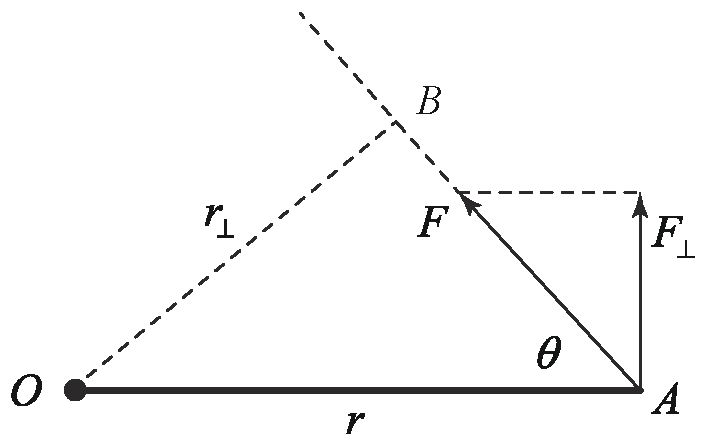
\includegraphics[width=0.5\linewidth]{images/static-force-9.pdf}
\caption{力矩的定义}
\label{fig:static-force-9}
\end{figure}


力的效果除了让物体有沿力的方向运动的趋势以外,对于刚体来说还会引起转动的趋,力学中用\emph{力矩}定量地描写力引起的转动效果。
对于如图所示的刚性杆,其一端固定于$O$点,在杆上$A$点处有外力$\vec{F}$的作用,它并不一定垂直于杆。
这时我们定义力$\vec{F}$相对于定点$O$的力矩$M$:
\begin{equation}
M = F r_{\perp} = F_\perp r = Fr\sin\theta
\end{equation}
各个量已在图中标出,其中$O$称为定义力矩的参考点,$A$为力的作用点,线段$OB$是从$O$到代表力的方向线段$OB$的垂线距离,它有一个专门的名称叫做\emph{力臂}。
除了具有一定的大小,力矩其实也是有方向的,对于定轴转动的物体来说,力矩的方向可以用它使物体有顺时针或逆时针转动的趋势来描写。
当一个物体受到多个力作用时,合力矩则是各个分力力矩之和。
因为力矩使物体有转动的趋势,所以处于静力平衡的系统中每个物体所受的力矩也必须为零。
需要注意的是和力不同,力矩的定义除了要指定力的大小和方向以外还有一个转动的参考点$O$,$O$点的选取并不一定必须在转动轴,甚至也不一定必须在受力物体上,无论将力矩的参考点选在何处,静力平衡均要求合力矩为零。
合理地选择参考点可以极大地简化受力分析的计算量。

总得来说处于平衡状态力学系统当中每个部分都需要它所受的合外力为零,相对任意参考点的合力矩为零。



%%%%%%%%%%%%%%%%%
\begin{example}

如图三根长度均为$l$的轻杆用铰链连接并固定在水平天花板上的$A、B$两点,$AB$两点相距$2l$,会在铰链$C$上悬挂一个质量为$m$的重物,要使$CD$ 杆保持水平,则在$D$点上应施加的最小力为多少?
\begin{flushright}
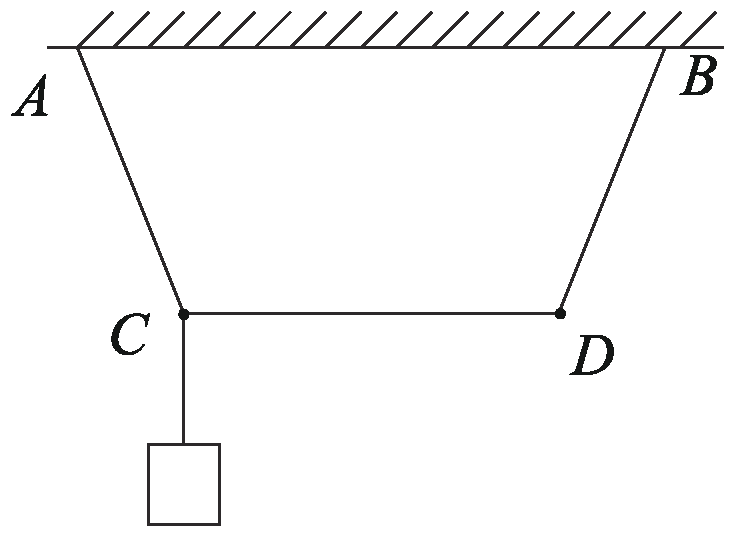
\includegraphics[width = 0.3\textwidth]{images/static-force-11.pdf} 
\end{flushright}
\tagged{student}{\vspace*{2cm}}
\begin{taggedblock}{teacher}
\vspace*{3cm}
\noindent
解析:对C和D的受力分析如上所示,C点受力平衡的条件给出:
\[
T_2 = \frac{\sqrt{3}}{3}mg,
\]
D要想受力平衡,那么$F$的最小值出现在图中所示的位置,这样
\[
F_{min} = \frac{mg}{2}
\]
\end{taggedblock}
\end{example}
%%%%%%%%%%%%%%%%%%%%%%


%%%%%%%%%%%%%%%%%
\begin{example}

求挡板在何角度时对小球的压力最小.
\begin{flushright}
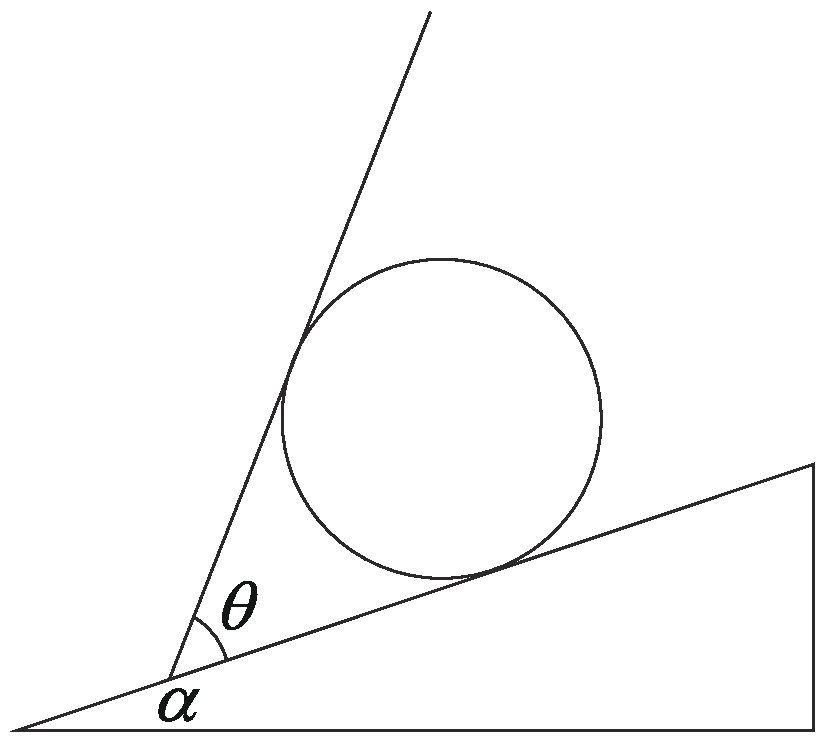
\includegraphics[width = 0.3\textwidth]{images/static-force-7.pdf} 
\end{flushright}
\tagged{student}{\vspace*{4cm}}
\begin{taggedblock}{teacher}
\noindent
解析:物体受力平衡的受力分析如上所示,其中重力大小方向均不变,斜面的支持力大小会变,但方向不变,挡板压力的大小方向均会变。
在挡板角度变化时通过画三力平衡的图可见当挡板与斜面垂直进对球的压力最小。
\end{taggedblock}
\end{example}
%%%%%%%%%%%%%%%%%%%%%%


%%%%%%%%%%%%%%%%%
\begin{example}
一质量为$m$的匀质球静止于倾角为$\theta_1$和$\theta_2$的两固定斜面之间,如图所示,设所有接触面都光滑,求斜面作用于球上的力。
\begin{flushright}
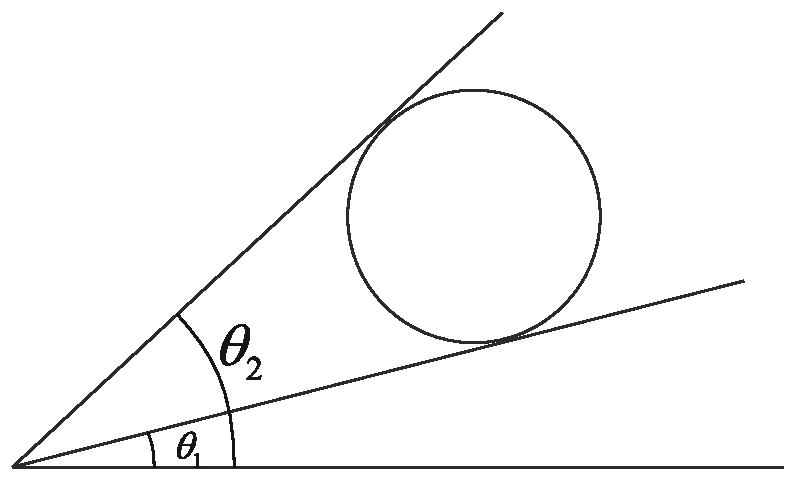
\includegraphics[width = 0.3\textwidth]{images/static-force-13.pdf} 
\end{flushright}

\tagged{student}{\vspace*{4cm}}
\begin{taggedblock}{teacher}

\vspace*{2cm}
\noindent
解析:如图所示,受力平衡方程给出:
\[N_1\sin\theta_1 = N_2\sin\theta_2,\qquad N_1\cos\theta_1 = mg+N_2\cos\theta_2,\]
两式联立求得可得
\[
N_1 = \frac{mg}{\cos\theta_1-\sin\theta_1\cos\theta_2},\qquad N_2 = \frac{mg\sin\theta_1}{\sin(\theta_2-\theta_1)}.
\]
\end{taggedblock}
\end{example}
%%%%%%%%%%%%%%%%%%%%%%





%%%%%%%%%%%%%%%%%
\begin{example}
两个质量为$M$,半径为$R$的相同圆球$A$和$B$,用两根长为$l$($l = 2R$)的绳悬挂于$O$点,在两球上另有一质量为$m$($m = nM$),半径为$r$(
$r=R/2$)的圆球$C$,如图,已知三球的表面
光滑,试讨论此系统处于平衡时,绳与竖直线的夹角$θ$与$n$的关系。
\begin{flushright}
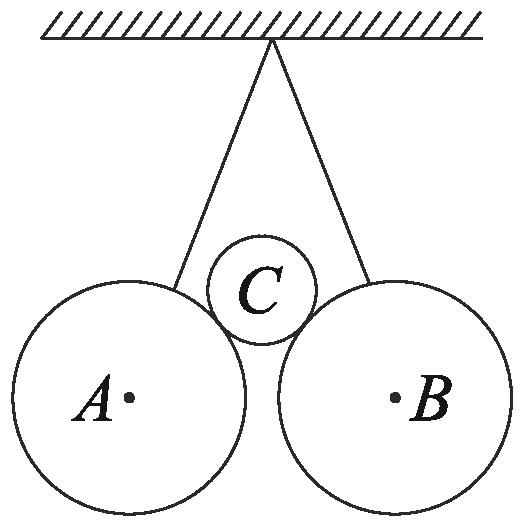
\includegraphics[width = 0.3\textwidth]{images/static-force-12.pdf} 
\end{flushright}

\tagged{student}{\vspace*{2cm}}
\begin{taggedblock}{teacher}

\vspace*{4cm}
\noindent
解析:受力分析如上所示,每个物体受力平衡。
对于A球我们有
\[
T\cos\theta = N\cos\alpha +Mg,\qquad T\sin\theta = N\sin\alpha,
\]
同样对于C球的平衡方程为
\[
2N\cos\alpha  = mg = nMg
\]
根据几何关系还有
\[
\frac{\sin\alpha}{\sin\theta} = \frac{3R}{\frac{3}{2}R} = 2,
\]
联立以上方程,最终解出夹角$\theta$满足:
\[
\sin\theta = \sqrt{\frac{4+4n-3n^2}{16(n+1)}}.
\]
又根据系统的特点分析可知当$\sin\theta<\frac{1}{3}$时两球实际上相碰,形成这样状态的条件
\[
\sin\theta\ge\frac{1}{3},\qquad n\le \frac{10+8\sqrt{10}}{27}\simeq 1.3
\]
综合以上的结果可知,当$C$质量较小$n<1.3$时$\sin\theta $由上式给出,$n=1.3$时两球相碰,而$n>1.3$时系统不能平衡。
\end{taggedblock}
\end{example}
%%%%%%%%%%%%%%%%%%%%%%










%%%%%%%%%%%%%%%%%
\begin{example}
如图所示一个均匀的质量为$m_1$、半径为$R$的球挂在天花板上$O$点处,从$O$点到球心的距离已知为$l$。
从同一点挂一个重物质量为$m_2$。
求图中$\theta$角的大小。
\begin{flushright}
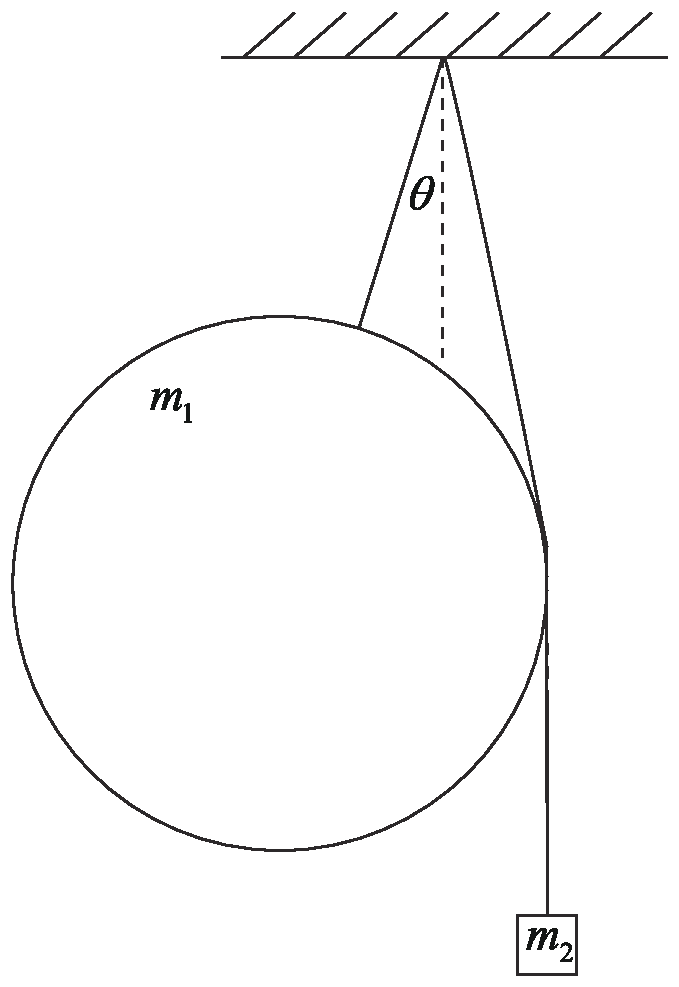
\includegraphics[width = 0.3\textwidth]{images/static-force-15.pdf} 
\end{flushright}
\tagged{student}{\vspace*{0cm}}
\begin{taggedblock}{teacher}
\noindent
解析:平衡时对$O$点力矩为零
\[
m_1gl\sin\theta = m_2g(R-l\sin\theta),\qquad \theta = \arcsin\left[\frac{m_2R}{(m_1+m_2)L}\right]
\]
\end{taggedblock}
\end{example}
%%%%%%%%%%%%%%%%%%%%%%




%%%%%%%%%%%%%%%%%
\begin{example}

有一个半径为$a$,高为$4a$,质量为$M$的两端开口的薄壁圆筒,现将筒竖放在光滑的水平面上,之后将半径为$r$,质量为$m$的两个完全相同的光滑圆球放入筒内而呈叠放状态,当$a< 2r < 2a$时,试求使圆筒不翻倒的条件。
\begin{flushright}
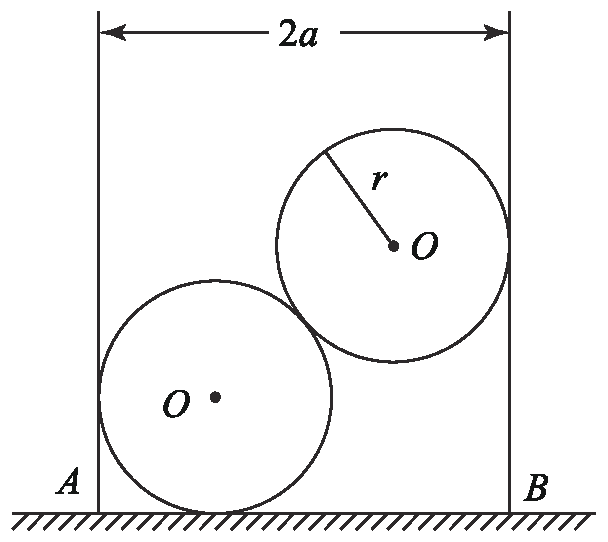
\includegraphics[width = 0.4\textwidth]{images/static-force-17.pdf} 
\end{flushright}
\tagged{student}{\vspace*{3cm}}
\begin{taggedblock}{teacher}

\vspace*{4cm}
\noindent
解析:假设系统处于图示的平衡状态,并令两球的质量逐渐增加。
当增加到一定程度以后圆筒就有可能翻倒,翻倒的临界点上,地面对圆筒的支持力将全部集中于右边的$B$点处。
受力分析指出两球和筒之间的作用力大小均为$N = mg\cot\theta$,$\theta$的定义如图所示,其大小可由几何关系决定:
\[
\cos\theta = \frac{a-r}{r}
\]

这样筒不翻倒需要使得对于$B$点压力的力矩小于重力力矩:
\[
N\cdot 2r\sin\theta \le mga,\qquad m\le M\frac{a}{2(a-r)}.
\]
\end{taggedblock}
\end{example}
%%%%%%%%%%%%%%%%%%%%%%


%%%%%%%%%%%%%%%%%
\begin{example}

有一轻木板,其自重可忽略,长为$l$,$A$端用铁链固定在竖直墙面上,另一端用水平绳拉住,板上依次放着三个圆柱体,其半径均为$r$,质量均为$m$,木板与墙面的夹角为$\theta$,一切摩擦均忽略不计,求水平绳对板的拉力$F$多大?
\begin{flushright}
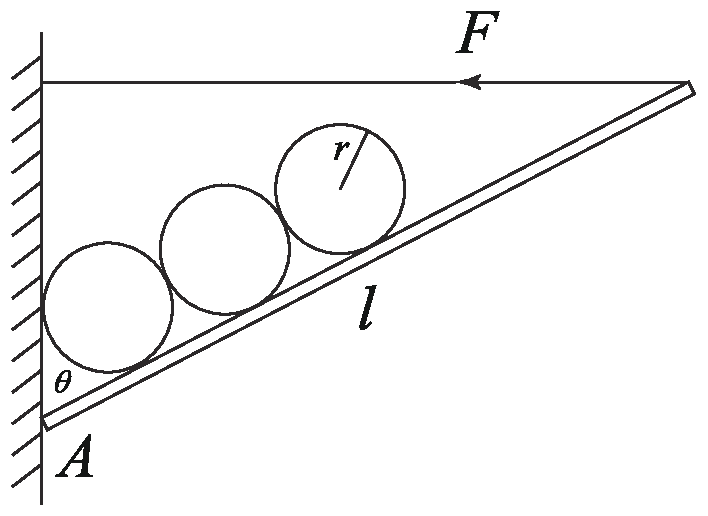
\includegraphics[width = 0.3\textwidth]{images/static-force-18.pdf} 
\end{flushright}
\tagged{student}{\vspace*{3cm}}
\begin{taggedblock}{teacher}
\noindent
解析:对每个球列受力平衡的方程,可以得到三个球对杆的压力分别为
\[
N_2=N_3 = mg\cos\theta,\qquad N_1 = mg\cos\theta+3mg\tan\theta\sin\theta.
\]
它们均垂直于杆,与A点的距离分别为
\[
l_1 = r\cot\frac{\theta}{2},\qquad l_2 = l_1+2r,\qquad l_3 = l_1+4r
\]
通过杆对A点转动力矩为零的条件可以解出拉力$F$
\end{taggedblock}
\end{example}
%%%%%%%%%%%%%%%%%%%%%%


%%%%%%%%%%%%%%%%%
\begin{example}


某机场候机楼结构简化图如图所示:候机楼侧壁是倾斜的,用钢索将两边斜壁系住,在钢索上有许多竖直短钢棒将屋面支撑在钢索上。
假设海边斜壁的质量为$m$,质量分布均匀;钢索与屋面(包括短钢棒)的总质量为 $2m$,在地面处用铰链与水平地面连接,钢索固定于斜壁上端以支撑整个屋面,钢索上端与斜壁的夹角为$30^\circ$;整个系统左右对称。
求斜壁对钢索的拉力的大小和斜壁与地面的夹角。
\begin{flushright}
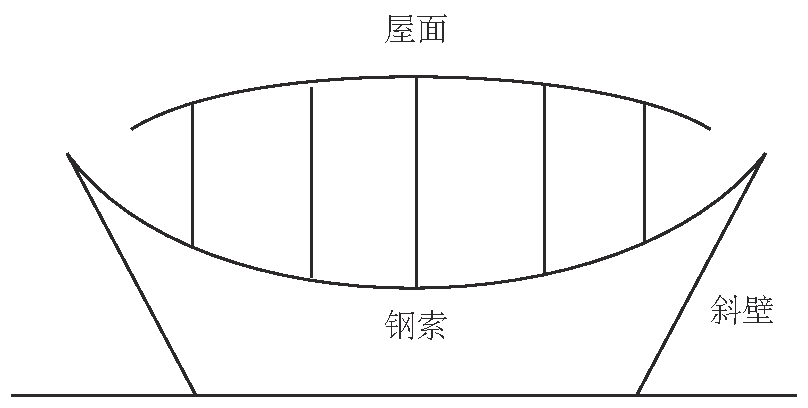
\includegraphics[width = 0.4\textwidth]{images/static-force-26.pdf} 
\end{flushright}
\tagged{student}{\vspace*{4cm}}
\begin{taggedblock}{teacher}
\noindent
解析:32届初赛
\end{taggedblock}
\end{example}
%%%%%%%%%%%%%%%%%%%%%%



\subsection{是否滑动?}

对于存在静摩擦力的平衡系统,求解平衡问题时有一个需要注意的地方就是静摩擦力并不是可以无限增加的,而是有一最大值。
通常来说静摩擦力的最大值与相互接触且有相对滑动趋物体之间接触面的性质以及相互之间的压力有关,其关系由式\ref{eqn: force-最大静摩擦}给出。

在处理此类问题时,一般来说首先假设两者间存在静摩擦力,在静摩擦力和其它所有力共同作用下保持平衡。
但在最后则需要做一个判断,假设的摩擦力$f$和两个挤压物体之间压力$N$的比值,如果$f< \mu N$,则可以保持平衡,但如果$f\ge \mu N$时就要小心了,两物体将会发生相对滑动。


\begin{figure}[htbp]
\begin{center}
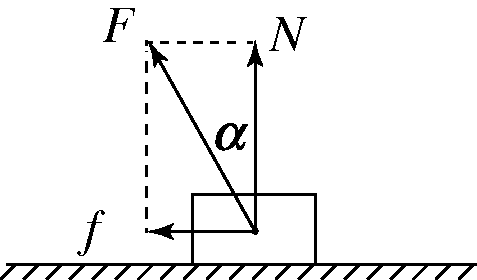
\includegraphics[width = 0.4\textwidth]{images/static-force-32.pdf} 
\caption{(a)有质量的绳中各部分张力不同,是位置的函数. (b)有质量且弯曲绳的受力分析}
\label{fig: force-支持力、摩擦力和全反力}
\end{center}
\end{figure}

除了用摩擦力和压力比值的方法判断是否滑动以外,还可以考虑可能滑动物体与接触表面之间压力和静摩擦力的合力,有时将其称为\emph{全反力}。
如图\ref{fig: force-支持力、摩擦力和全反力}所示的$F$就是全反力,它与接触面垂线的夹角$\alpha$是标志全反力的一个重要的物理量。
从图中可以看出,当$\alpha$为已知时,压力$N = F\cos\alpha$,摩擦力$f=F\sin\alpha$,所以不发生滑动的条件此时就变成了
\begin{equation}
\sin \alpha < \mu\cos\alpha,\qquad \text{或},\qquad \tan\alpha < \mu,
\end{equation}
也就是说全反力和法线夹角的正切小于摩擦系数时,无相对滑动,反之则不可能相对静止。


%%%%%%%%%%%%%%%%%
\begin{example}
木箱质量为$M$,与地面间的动摩擦因数为$\mu$,用斜向上的力$F$拉木箱使之沿水平地面匀速前进,如图所示,问角$\alpha$为何值时拉力$F$最小?
这个最小值为多大?
\begin{flushright}
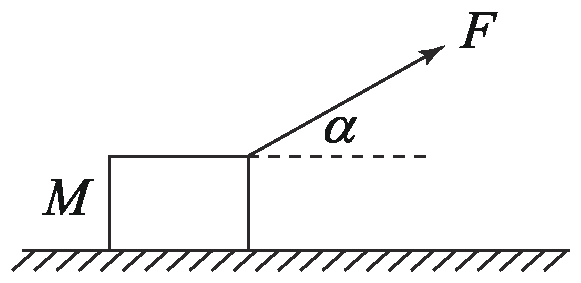
\includegraphics[width = 0.3\textwidth]{images/static-force-5.pdf} 
\end{flushright}

\tagged{student}{\vspace*{1cm}}
\begin{taggedblock}{teacher}

\vspace*{3cm}
\noindent
解析:物体可看成受三个力的作用:重力、拉力和地面的全反力,匀速滑动意味着三力平衡。
由于是滑动所以全反力与平面垂线方向的夹角刚好是摩擦角,在这个条件下很容易判断出拉力的最小值
\[
F_{min} = mg\sin\alpha = mg\frac{\mu}{\sqrt{1+\mu^2}}
\]
\end{taggedblock}
\end{example}
%%%%%%%%%%%%%%%%%%%%%%


%%%%%%%%%%%%%%%%%
\begin{example}
筷子夹鸡蛋(只考虑在水平光滑桌面上)的摩擦紧锁问题:设筷子与鸡蛋的摩擦系数为$\mu$,求筷子多大角度时在水平桌面上始终不会把鸡蛋滑出。
\begin{flushright}
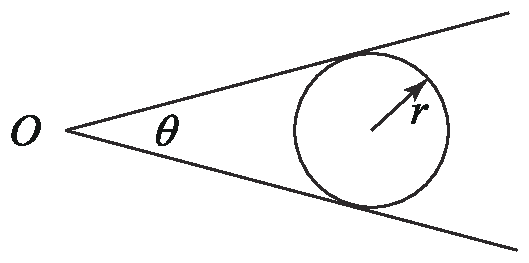
\includegraphics[width = 0.4\textwidth]{images/static-force-4.pdf} 
\end{flushright}
\tagged{student}{\vspace*{2cm}}
\begin{taggedblock}{teacher}

\vspace*{2cm}
\noindent
解析:蛋受两个全反力,如需平衡需要两个力共线。
这样要求全反力与筷子垂线的夹角小于摩擦角
\[
\mu>\tan\frac{\theta}{2}.
\]
\end{taggedblock}
\end{example}
%%%%%%%%%%%%%%%%%%%%%%



%%%%%%%%%%%%%%%%%
\begin{example}
有一长$l$质量为$M$的均匀杆$AB$,$A$顶端竖直的粗糙墙壁上,杆端与墙间的摩擦系数为$\mu$,$B$端用一强度足够而不可伸长的绳悬挂,绳的另一端固定在墙壁$C$点,木杆呈水平状态,绳与杆的夹角为$\theta$,求杆能保持平衡时$\mu$与$\theta$应满足的条件。
杆保持平衡时,杆上有一点$P$存在,若$A$与$P$点间挂一重物,则$M$足够大可以破坏平衡了,而在$PB$间任一点悬挂任意重物均不能破坏平衡。求$PA$距离$x$。

\begin{flushright}
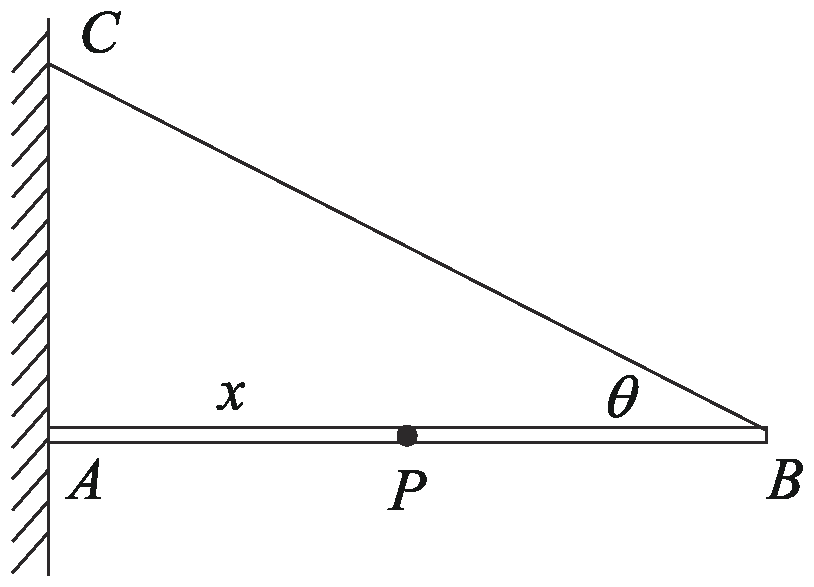
\includegraphics[width = 0.3\textwidth]{images/static-force-16.pdf} 
\end{flushright}

\tagged{student}{\vspace*{3cm}}
\begin{taggedblock}{teacher}
\vspace*{2cm}

\noindent
解析:受力分析如上所示,要想平衡需要三力共点,通过摩擦角可知需要满足条件
\[
\mu\ge \tan\theta.
\]
当物体足够重了以后,杆的重力可忽略不计,如果全反力与杆的夹角无论多重都小于摩擦角时我们有$P$点到$A$的距离必须满足
\[
x>\frac{\tan\theta}{\tan\theta +\mu}l
\]
\end{taggedblock}
\end{example}
%%%%%%%%%%%%%%%%%%%%%%


%%%%%%%%%%%%%%%%%
\begin{example}

如图,一人对一均匀细杆的一端施力,力的方向总与杆垂直,要将杆从地板上无滑动地慢慢抬到竖直位置,试求杆与地板间的静摩擦因数至少应为多大?
\begin{flushright}
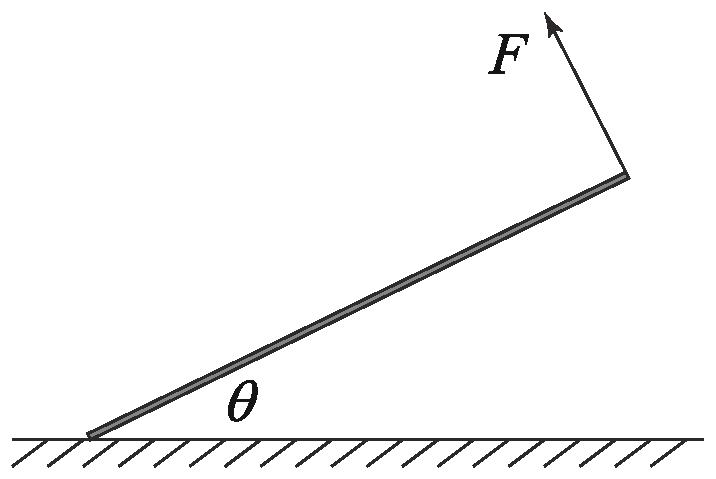
\includegraphics[width = 0.3\textwidth]{images/static-force-21.pdf} 
\end{flushright}
\tagged{student}{\vspace*{0cm}}
\begin{taggedblock}{teacher}

\vspace*{3cm}

\noindent
解析:受力分析如上,两个方向受力平衡,力矩平衡方程联立可得在某一给定角度$\theta$下,摩擦力$f$与支持力$N$的比值
\[
\frac{f}{N} = \frac{\sin\theta\cos\theta}{1-2\cos^2\theta},
\]
在$\theta$角变化的过程中两者比值的最小值出现在
\end{taggedblock}
\end{example}
%%%%%%%%%%%%%%%%%%%%%%


%%%%%%%%%%%%%%%%%
\begin{example}
质量均为$m$的两环$A$、$B$用长为$a$的细线相连在水平杆上,在细线的中点拴有一质量为$M$的物块$C$,$A、B$环与杆间的静摩擦系数为$\mu$,求平衡情况下的两环的最大距离$x$。
\begin{flushright}
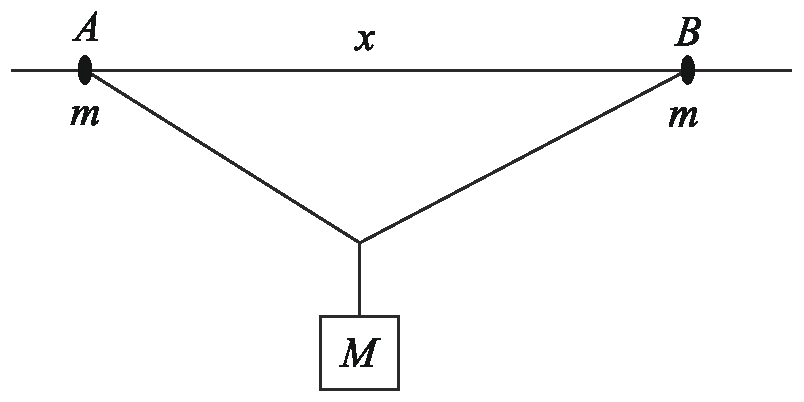
\includegraphics[width = 0.4\textwidth]{images/static-force-14.pdf} 
\end{flushright}

\tagged{student}{\vspace*{4cm}}
\begin{taggedblock}{teacher}
\noindent
解析:
\end{taggedblock}
\end{example}
%%%%%%%%%%%%%%%%%%%%%%

\subsection{有质量绳的情况}
之前问题中的绳一般来说总是取无质量的极限,这种情况下当绳的拉力不为零,包含有绳的系统处于平衡状态时绳均为直线(多数情况下绳的伸长也被忽略),并且两端的拉力相等。
但实际上对于很多问题来讲,绳的质量和它的形变是不能忽略不计的,例如桥梁上的斜拉索,它一方向负责承担桥梁其它部分的重量,另一方面必须采用足够强度的材料以保证其可靠性,这时其自重就不可忽略不计。
\begin{figure}[htbp]
\begin{center}
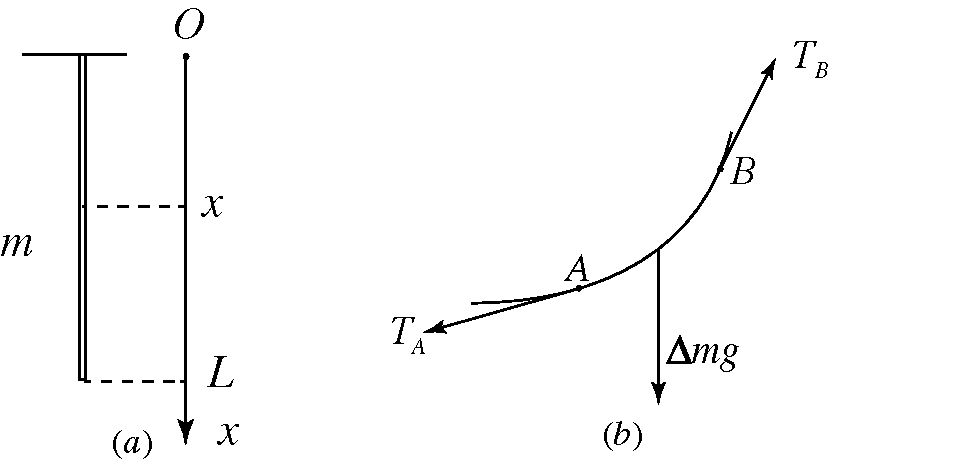
\includegraphics[width = 0.7\textwidth]{images/static-force-29.pdf} 
\caption{(a)有质量的绳中各部分张力不同,是位置的函数. (b)有质量且弯曲绳的受力分析}
\label{fig: force-有质量的绳中各部分张力不同,是位置的函数}
\end{center}
\end{figure}




当考虑可变形物体的质量时,其内部各部分之间的作用力将不再相同,除了承担外部的受力以外,其自重也会改变不同位置处的受力。
最简单的例子如图\ref{fig: force-有质量的绳中各部分张力不同,是位置的函数}(a)所示,一根质量为$m$,长度为$L$的均匀绳静止悬挂于$O$点,建立一个原点在$O$点,竖直向下的坐标系$Ox$,这时绳中张力$T$就不再是常数,而是坐标$x$的函数。
在某一$x$点处的张力用来平衡处于其下部绳的重力,简单的分析可知绳中张力满足
\[T(x) = mg(L-x)\]
在绳的顶端,也就是$x=L$处很明显张力为零。
在更复杂的情况下不但绳中张力不同,绳还会发生弯曲。
这时任何一点处的张力的方向是绳在该处的切线方向,此时如果绳的质量不可忽略,需要取绳中极小一段做为研究对象,两端的张力在水平方向上平衡,而在竖直方向上与该段绳的重力平衡,如图\ref{fig: force-有质量的绳中各部分张力不同,是位置的函数}(b)中那样。



%%%%%%%%%%%%%%%%%
\begin{example}
如图所示,一个顶角为$\alpha$的光滑圆椎体,一个质量为$m$,原长为$L_0$,劲度系数为$k$的弹性绳处于平衡状态,所有部分均处于同一水平面上,求平衡绳到椎顶的距离。
\begin{flushright}
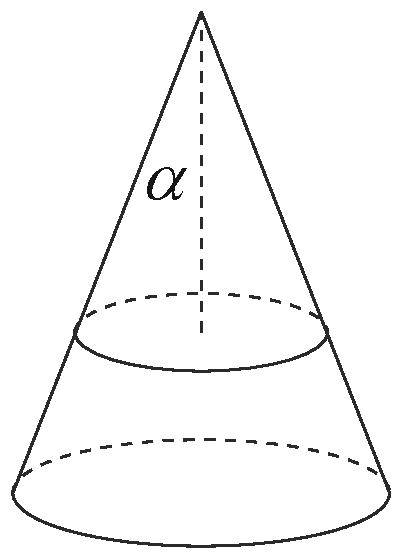
\includegraphics[width = 0.2\textwidth]{images/static-force-25.pdf} 
\end{flushright}

\tagged{student}{\vspace*{2cm}}
\begin{taggedblock}{teacher}
\noindent
解析:当距离为$h$时绳的长度$L = 2\pi h\tan\alpha$,这样它的伸长量$\Delta L = L-L_0 =L = 2\pi h\tan\alpha-L_0 $,由于弹性系数为已知所以绳中的张力
\[
T = k\Delta L = k( 2\pi h\tan\alpha-L_0).
\]
取绳中张角为$\Delta\theta$的一小段为研究对象,质量$\Delta m = \frac{\Delta \theta}{2\pi}m$,这一小段绳在重力,椎体支持力以及张力共同作用下平衡:
\[
mg\cos\alpha = k( 2\pi h\tan\alpha-L_0)\sin\alpha,
\]
整理可得
\[
h = \frac{\frac{mg}{k}\cot\alpha+L_0}{2\pi\tan\alpha}.
\]
\end{taggedblock}
\end{example}
%%%%%%%%%%%%%%%%%%%%%%

%%%%%%%%%%%%%%%%%%%%%%%%%%%%%%%%%%
\begin{example}
有一个固定在水平面上半径为$R$的半圆柱形光滑物体和一根质量为$m$,长为$ \frac{\pi R}{2}$的均匀绳。
它们处于如图所示位置的平衡状态,求维持平衡作用于绳顶端水平向左力$F$的大小。
\begin{flushright}
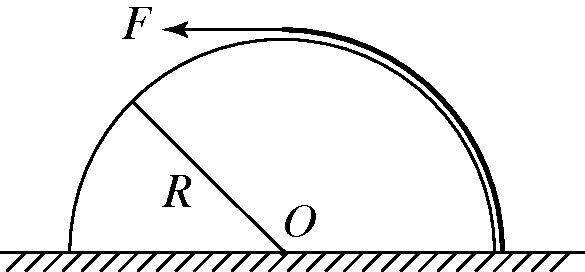
\includegraphics[width=0.4\textwidth]{images/static-force-31.pdf}
\end{flushright}
\tagged{student}{\vspace*{4cm}}
\begin{taggedblock}{teacher}

\vspace*{3cm}
\noindent
解析:取上图所示$\theta$到$\theta+\Delta \theta$当中的一小段,受力分析已经标出。
它要想受力平衡需要满足
\[
\Delta T = \frac{\Delta \theta}{\pi/2}Mg\cos\theta 
\]
从最下面加到最上面我们有
\[
T(\frac{\pi}{2}) = \sum\Delta T = \frac{2}{\pi}mg
\]
\end{taggedblock}
\end{example}
%%%%%%%%%%%%%%%%%%%%%%%%%%

%%%%%%%%%%%%%%%%%
\begin{example}
质量为$m$,长为$l$的均匀光滑细绳,穿过半径为$R$的光滑滑轮并搭在轮上,求绳上的最大张力。
\begin{flushright}
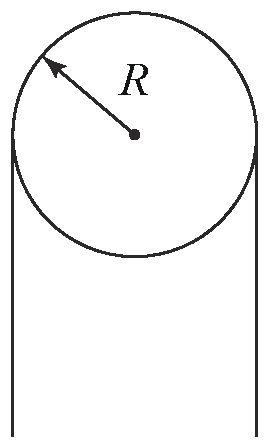
\includegraphics[width = 0.2\textwidth]{images/static-force-20.pdf} 
\end{flushright}
\tagged{student}{\vspace*{3cm}}
\begin{taggedblock}{teacher}
\noindent
解析:和前一问一样的思路,通过分割小段以后受力分析可得最高点的张力最大,最大值为
\[
T_{max} = \frac{l-(\pi-2)R}{2l}mg.
\]
\end{taggedblock}
\end{example}
%%%%%%%%%%%%%%%%%%%%%%

%%%%%%%%%%%%%%%%%
\begin{example}

半径为$R$的刚性球固定在水平桌面上,有一个质量为$M$的圆环状均匀弹性绳圈,原长$2\pi a$,$a=R/2$。
绳圈的弹性系数为$k$(绳圈伸长$s$时,绳中弹性张力为$ks$)。
将绳圈从球的正上方轻放到球上,并用手扶着绳圈使之保持水平并最后停留在某个静力平衡位置,设此时绳圈的长度为$2\pi b,b = \sqrt{2}a$,考虑重力,忽略摩擦,求绳圈的弹性系数$k$?
(用$M$、$R$、$g$表示,$g$为重力加速度)
\begin{flushright}
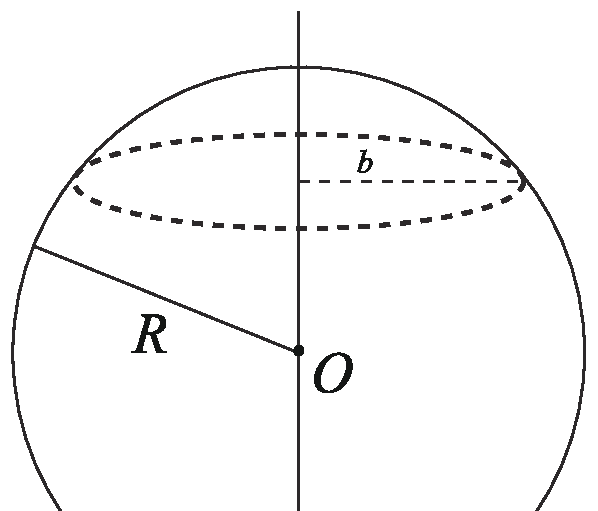
\includegraphics[width = 0.3\textwidth]{images/static-force-19.pdf} 
\end{flushright}
\tagged{student}{\vspace*{4cm}}
\begin{taggedblock}{teacher}
\noindent
解析:通过给出的信息可知平衡时绳中的张力
\[
T = (\sqrt{2}-1)k\pi R,
\]
取绳上张角很小的一段进行分析,可得它的平衡条件为
\[
T = \frac{mg}{2\pi},\qquad k = \frac{mg}{2(\sqrt{2}-1)\pi^2R}
\]
\end{taggedblock}
\end{example}
%%%%%%%%%%%%%%%%%%%%%%




%%%%%%%%%%%%%%%%%%%%%%%%%%%%%%%%%%
\begin{example}
【思考题】一根长度为$L$,质量为$m$的均匀绳两端固定在处于同的水平面上相距$d<L$的$A$、$B$两点,你能够用何种方法决定平衡以后绳的形状。
\begin{flushright}
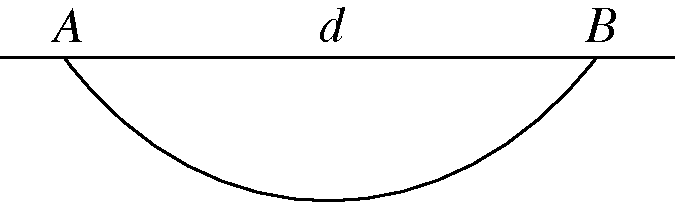
\includegraphics[width=0.4\textwidth]{images/static-force-30.pdf}
\end{flushright}
\tagged{student}{\vspace*{4cm}}
\begin{taggedblock}{teacher}
\noindent
解析:悬链线,对每一段受力分析相对比较麻烦,可以用平衡时重心最低来尝试求解。
\end{taggedblock}
\end{example}
%%%%%%%%%%%%%%%%%%%%%%%%%%

\subsection{平衡的稳定性}
仅仅解出受力平衡的方程有时候并不见得能够给出力学系统平衡位置,真正的平衡状态除了要考虑平衡本身以外,还需要考虑平衡的稳定性。
如下图所示,同样的两根竖直放置的杆,第一根杆由其顶部的线悬挂在固定点处,另一根则放置于水平桌面上。
两杆受到与重力方向相反的拉力或桌面的支持力,满足静力学平衡的基本条件。但简单的分析可知,第一根杆是稳定的而第二根杆则必然不稳定,即这样的平衡状态实际上是不可能发生的。

\begin{figure}[htbp]
\begin{center}
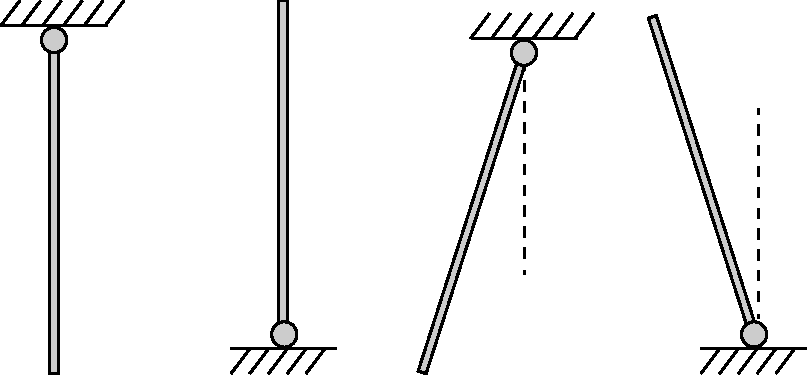
\includegraphics[width=0.6\textwidth]{images/static-force-28}
\caption{稳定和不稳定平衡}
\label{default}
\end{center}
\end{figure}

造成这一现象的原因很简单,处于力学平衡的系统不可避免地会受到各种影响。
如果对平衡状态产生一个扰动,则系统将会或多或少地偏离期平衡位置,一般来说其受力也会随之变化。
当平衡系统偏离了平衡位置以后所受外力的方向指向平衡位置,或者更一般的,合外力的趋势是使其向原有的平衡状态运动,那么这种平衡状态就是\emph{稳定}的。
例如垂直悬挂的杆,当稍稍偏垂线方向一个角度以后,重力产生相对悬挂点的力矩的方向有使偏离角变小的趋势,所以这样的平衡状态是稳定的。
反之,当偏离平衡状态以后的合力方向或效果使相对于平衡位置的偏离量变大,这样的平衡状态实际上就是\emph{不稳定}的,例如竖直放置的那根杆所表现出来的那样。

一个力学系统稳定性的判断对解决静力学问题也是至关重要的,平衡的稳定性并不能通过受力平衡方程直接得到,而是需要进一步的判断。
经过大量的计算而得到一个不稳定的平衡位置有时也是无意义的,因为这样的状态实际上并不可能出现,如果将这样的结果应用到工程当中甚至会造成破坏性的结果。
一般来说平衡的稳定性可以通过定性的分析进行判断,但有时也需要一定程度的定量计算。


%%%%%%%%%%%%%%%%%
\begin{example}
一根质量为$m$的均匀杆,长为$L$,下端可绕固定水平轴转动.有两根水平弹簧,劲度系数相同,拴在杆的上端,使其处于竖直位置.问:弹簧的劲度系数$k$为何值,才能使杆处于稳定平衡?
\begin{flushright}
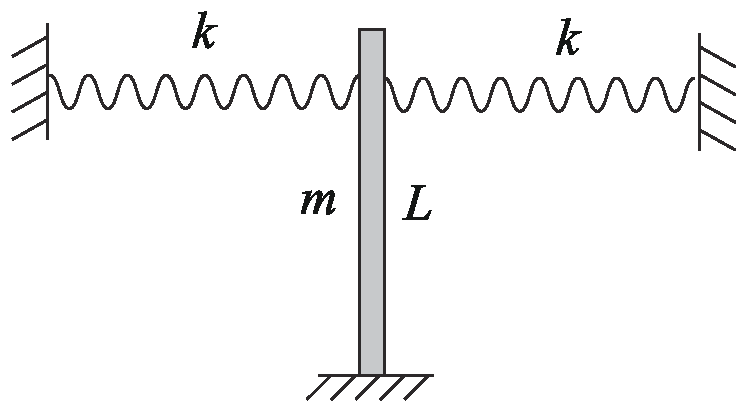
\includegraphics[width = 0.4\textwidth]{images/static-force-23.pdf} 
\end{flushright}
\tagged{student}{\vspace*{2cm}}
\begin{taggedblock}{teacher}
\noindent
解析:将杆稍向右移动一点,角度为$\Delta \theta$。
这时每根弹簧的形变量都是$L\Delta \theta$,能够提供向左转动的力矩为$2kL^2\Delta \theta$,与此同时重力会带来一个向右转动的力矩,大小则是$\frac{1}{2}mgL\Delta\theta$,要想实现稳定平衡,要求
\[
2kL^2>\frac{1}{2}mgL,\qquad k>\frac{mg}{4L}.
\]
\end{taggedblock}
\end{example}
%%%%%%%%%%%%%%%%%%%%%%

%%%%%%%%%%%%%%%%%
\begin{example}

两根长度均为$L$,质量忽略不计的刚性轻杆固定在竖直平面内,顶端由铰链连接并固定有一个质量为$M$的质点。
下端连接一根劲度系数为$k$,原长为0的轻弹簧,求平衡时杆与垂线的夹角$\theta$。
\begin{flushright}
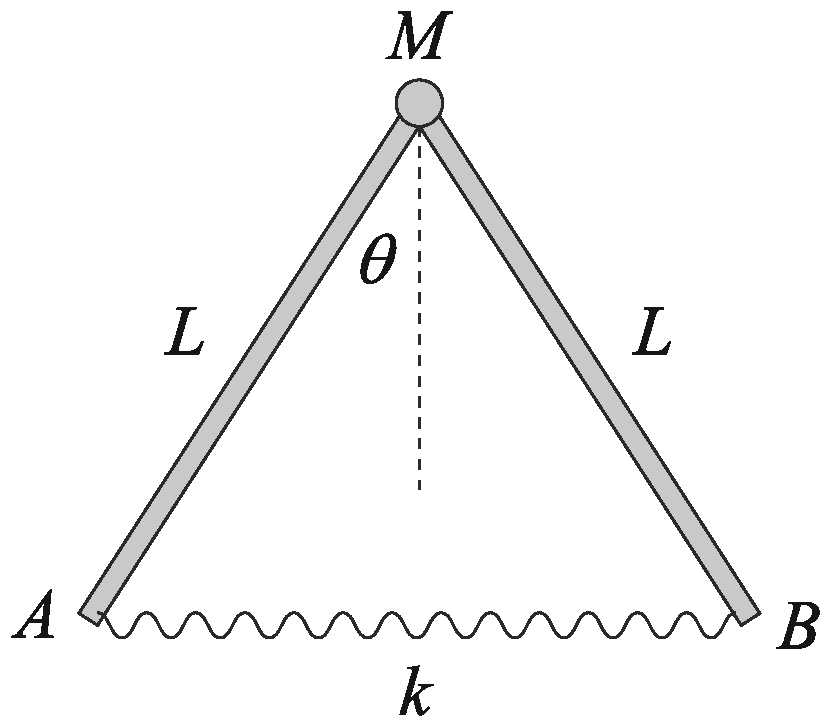
\includegraphics[width = 0.3\textwidth]{images/static-force-24.pdf} 
\end{flushright}
\tagged{student}{\vspace*{4cm}}
\begin{taggedblock}{teacher}
\noindent
解析:通过受力分析容易得到平衡时
\[
\cos\theta = \frac{mg}{4kl},\qquad \text{或者} \qquad \sin\theta = 0
\]
但其实这个结果当中的第一个是不稳定平衡,在那样的平衡状态下只要$\theta$有微小的变化,系统就是持续地偏离,这一点可通过受力分析得到。
\end{taggedblock}
\end{example}
%%%%%%%%%%%%%%%%%%%%%%
%%%%%%%%%%%%%%%%%
\begin{example}
一根长为$L$的杆一端靠与竖直墙面,另一端靠在曲面上,此水平轴为$x$,竖直轴为$y$,要杆在任何位置都平衡,求曲面的截面满足的条件。
\begin{flushright}
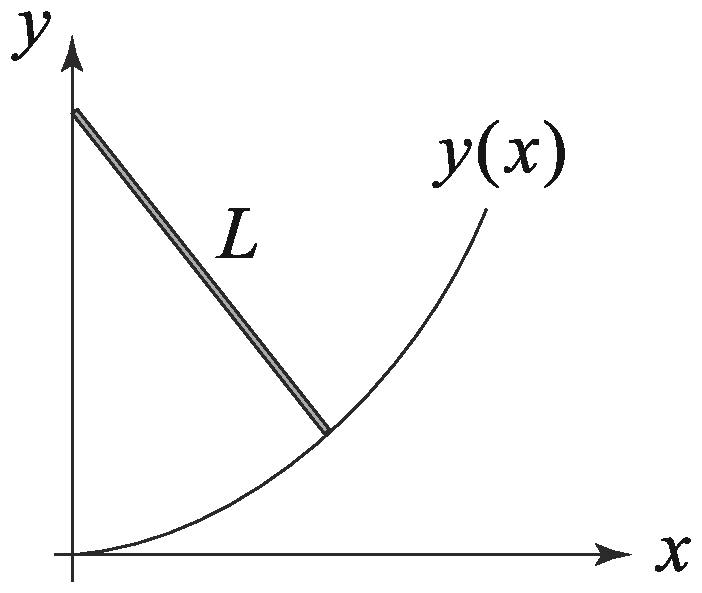
\includegraphics[width = 0.3\textwidth]{images/static-force-22.pdf} 
\end{flushright}

\tagged{student}{\vspace*{4cm}}
\begin{taggedblock}{teacher}
\noindent
解析:要想时刻保持平衡,那么就必须使得杆在不同位置时重心的高度保持不变。
设在任意位置上杆与$y$轴的交点纵坐标为$Y$,与曲面交点的坐标则是$(x,y)$,它们之间满足
\[
x^2+(Y-y)^2=l^2
\]
这时杆重心的纵坐标为$y_c = \frac{y+Y}{2}$,它必须与杆完全处于竖直位置时重心的高度一致,从这个条件可知重心的高度必为$\frac{l}{2}$,也就是
\[
\frac{y+Y}{2} = \frac{l}{2},\qquad Y = l-y
\]
将它代入第一个式子就有曲面截面满足的方程:
\[
x^2+(l-2y)^2 = l^2
\]
\end{taggedblock}
\end{example}
%%%%%%%%%%%%%%%%%%%%%%


%%%%%%%%%%%%%%%%%
\begin{example}
【思考题】如图,一个圆形的“碗”半径为$R$,一个小球半径为$r$。
小球不是匀质的,请问小球重心高度$h$为多大时候才会形成稳定平衡。
如果半径$R$不断增大,会怎样?增大到无穷大会怎样?再进一步增大会怎样?
\begin{flushright}
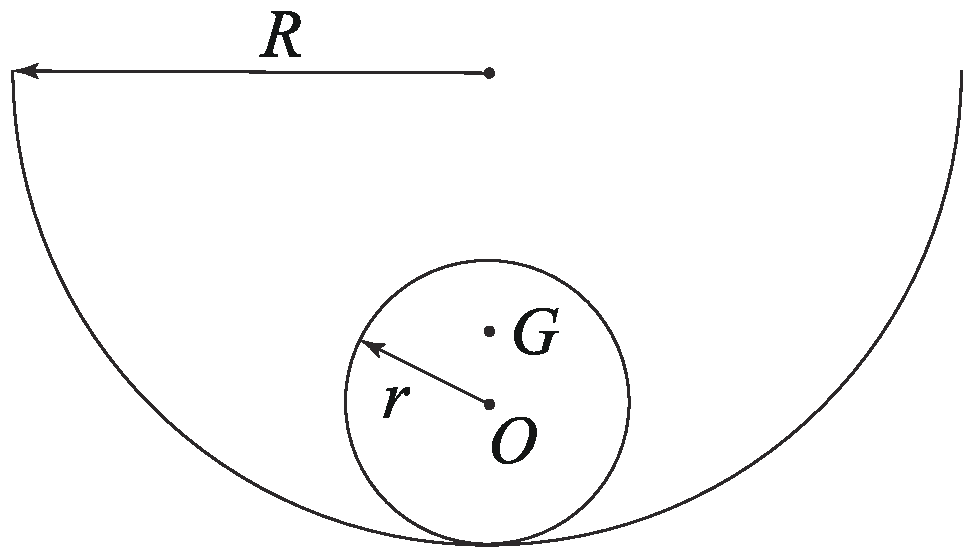
\includegraphics[width = 0.4\textwidth]{images/static-force-27.pdf} 
\end{flushright}
\tagged{student}{\vspace*{3cm}}
\begin{taggedblock}{teacher}
解析:$h<\frac{rR}{R-r}$是稳定的。R增加到无穷大,h<r就是稳定的。

\end{taggedblock}
\end{example}
%%%%%%%%%%%%%%%%%%%%%%
